
\documentclass{article}
\usepackage[top=10em]{geometry}
\usepackage{amsmath}
\usepackage{tikz}
\usepackage{tikz-qtree,tikz-qtree-compat}
\usepackage{graphicx}
\usepackage[margin=1cm]{caption}

\title{Compressive Saliency Sensing: sampling near the edges}
\date{}
\author{Scott Sievert, \texttt{sieve121@umn.edu}}

\begin{document}


    \maketitle
    \tableofcontents
    \hrulefill

    \section{One Dimension}
        In one dimension, we do not have a tree like we do in the two dimension case. Instead of having three branches like the 2D case, we have two branches at each node.

        \subsection{Approximating the Wavelet transform}

          
          Lets say we have an $n$ dimensional signal: $x = (x_1,\ldots,x_n)^T$. We can take the wavelet transform of this signal, $w$, using $x = h w$, where $h$ is the wavelet matrix (in our case, the simple Haar matrix).

            The terms in $w$ correspond to different frequency components, and the latter terms correspond to higher frequencies. We only care about these terms if we're close to an edge, since that's where high frequency terms are. There's no need to approximate a DC or constant term with high frequency.

            So let's say we're only interested in the top $m$ terms of $w$, since what's specified when we approximate the wavelet. Since we only care about the upper portions of $w$, we can get rid of the corresponding rows for $h$.

            $$ 
                \begin{bmatrix}  
                    h_{1,1} & h_{1,2} &h_{1,3} &h_{1,4} \\
                    h_{2,1} & h_{2,2} &h_{2,3} &h_{2,4} \\
                    h_{3,1} & h_{3,2} &h_{3,3} &h_{3,4} \\
                    h_{4,1} & h_{4,2} &h_{4,3} &h_{4,4} \\
                
                \end{bmatrix}
                \begin{bmatrix}
                    w_1 \\ w_2 \\ w_3 \\ w_4
                \end{bmatrix}
            $$

            Since we only care about the first two entries of $w$ ($m=2$), we can write

            $$
                \begin{bmatrix}  
                    h_{1,1} & h_{1,2}  \\
                    h_{2,1} & h_{2,2}  \\
                    h_{3,1} & h_{3,2}  \\
                    h_{4,1} & h_{4,2}  \\
                
                \end{bmatrix}
                \begin{bmatrix}
                    w_1 \\ w_2 \\ 
                \end{bmatrix}
            $$

            And, saying we didn't sample at index number 2, we can write

            $$
                \begin{bmatrix}  
                    h_{1,1} & h_{1,2}  \\
                    h_{3,1} & h_{3,2}  \\
                    h_{4,1} & h_{4,2}  \\
                
                \end{bmatrix}
                \begin{bmatrix}
                    w_1 \\ w_2 \\ 
                \end{bmatrix}
            $$

            Carrying out that matrix multiplication, or solving a linear system of equations, will approximate the wavelet coefficients.

        \subsection{Going between the wavelet and time indices}

            We know that $h^{-1} x = w $. Since we know that  $h_{i, j} = 0$, we know that $x_j$ won't matter for the $i$th element of $w$.
            
        \subsection{The actual reconstruction}

        We approximate the first $m=2^{level}$ terms of the wavelet transform. If these coefficients are large enough ($|w_i|> \lambda$), we sample more at the indices corresponding to that wavelet location.


    \section{Two Dimensions}
        %\subsection{The wavelet transform with matrices}
            %For two dimensions, we have to do the wavelet transform on each row and column recursively. In matrix language, it's $w_{level} = c x r$. To get it to higher dimensions, we can use the identity matrix and change the upper left corner.
            %$$w = I_c (c x r) I_r $$
            
            %We then want $mx = w$. Since we now know always know $x$ and now know $w$, we can easily find $m$: $$ m = w x^{-1}$$

            %But, I just had an ``aha!'' moment. We don't have to find $w$ with matrices. We can just use my handy-dandy function, \texttt{dwt2\_full(x)}.

            %This isn't the best method. Since we're much of our image is the same, the matrix is singular (or at least close to it). We need to find another method to both approximate the transform and figure out which indices are important.
            
        \subsection{Approximating the wavelet transform}
            %We can easily get $m$ using \texttt{dwt2\_full}. It's then the same problem as in one dimension: solve a linear system. Since you only care about the coarse wavelet coefficients, delete the rows $m$ that give you those. Also delete the columns that you don't sample at.
            I think this is the same as in 1D: we have to delete the appropriate rows and columns.Since we have $w = c x r$, and we only care about $m$ terms of $w$, we can delete the last $n-m$ rows of $c$ and the last $n-m$ columns of $r$.

            Just making sure the sizes check out:
            $$ w^{m\times m} = c^{m\times n} x^{n \times n} r^{n \times m} $$
            $$ w^{m\times m} = temp^{m \times n} r^{n \times m} $$
            $$ w^{m\times m} = temp^{m \times m}$$


            That was assuming that $x$ was fully sampled. Since we're undersampling, we'll have to delete those entries of $x$, columns of $c$ and rows of $r$.


        \subsection{Which indices are important?}
            Initially, I thought that the wavelet transform had to be recursive. That makes it really tricky for the indices -- you would have to make \texttt{dwt\_ind} functions, and keep doing it. 

            But after I talked to Ashkay, I learned that you can do the full wavelet transform on each row then each wavelet transform on each column. That makes this function trivial: it's just a matter of indexing. 

        \subsection{The reconstruction}
            In the wavelet domain, we have a tree that corresponds to the image. An example is in Figure~\ref{fig:tree}. The upper levels of the tree represent the lower frequency terms. Since there's no need to closely sample a low frequency term, we only sample where there are high frequencies. 

            We know that if any of these ``branches'' are close enough to zero ($|x| < \lambda$) that all of it's child branches are close enough to 0 as well. Therefore, we only look at where the branches are not close enough to zero ($|x| > \lambda$). As we go further down the branch, we form a better approximation of the wavelet transform.
            
            \begin{figure}
            	\hspace{8em}
                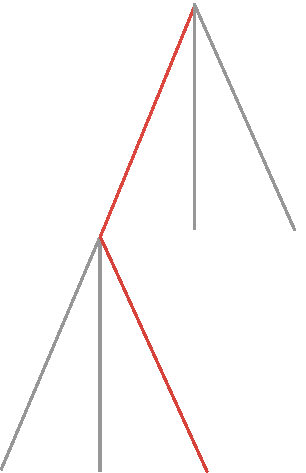
\includegraphics[angle=90]{tree}
                \caption{A visualization of a tree. The wavelet transform only includes high frequency components in the lower "branches", so we only go deeper in the tree if necessary. Each level of the wavelet contains horizontal, vertical and diagonal branches. }
                \label{fig:tree}
            \end{figure}
            
            Where we choose to look (or where we sample) is near the edges. The wavelet transform is zero for a constant: it has no high frequency terms.



\end{document}





































